% --------------------------------------------------------------
% This is all preamble stuff that you don't have to worry about.
% Head down to where it says "Start here"
% --------------------------------------------------------------
 
\documentclass[12pt]{article}

\usepackage[margin=1in]{geometry} 
\usepackage{amsmath,amsthm,amssymb,listings,xcolor,graphicx, subfig, subcaption, enumerate,framed}
 
\newenvironment{solution}{\begin{proof}[Solution]}{\end{proof}}

\definecolor{codegreen}{rgb}{0,0.6,0}
\definecolor{codegray}{rgb}{0.5,0.5,0.5}
\definecolor{codepurple}{rgb}{0.58,0,0.82}
\definecolor{backcolour}{rgb}{0.97,0.97,0.97}
\lstdefinestyle{pystyle}{
    backgroundcolor=\color{backcolour},   
    commentstyle=\color{codegreen},
    keywordstyle=\color{magenta},
    numberstyle=\tiny\color{codegray},
    stringstyle=\color{codepurple},
    basicstyle=\ttfamily\small,
    breakatwhitespace=false,         
    breaklines=true,                 
    captionpos=b,                    
    keepspaces=true,                 
    numbers=left,                    
    numbersep=5pt,                  
    showspaces=false,                
    showstringspaces=false,
    showtabs=false,                  
    tabsize=2
}
\lstset{style=pystyle}

\graphicspath{{./figures}}
 
\begin{document}
 
\title{Homework 6: Wavelets and Wavelet Filterbanks}
\author{Matthew Luyten\\
ECE6250}

\maketitle

\begin{enumerate}
\item[Problem 6.1] Summary and Context of Wavelets and Wavelet Filterbanks

This week, we learned more about wavelets and wavelet filterbanks. This topic
feels like a logical progression from the 2D dicrete cosine transform since 
wavelets are often used to represent images. For example, the JPEG 2000 algorithm
used wavelets as an alternative to the original 1992 JPEG DCT algorithm.

Wavelets are another important extension of the groundwork set by the last month of
class regarding orthogonal projections. This adds one more transform tool to the DSP 
tool belt. One interresting application is the 'free' filterbank that is provided
when performing a wavelet transform. This makes the wavelet transform very
advantageous when perorming filtering and compression in the same step. This also
provides an intiutive and general framework for wavelet and scaling functions.

\newpage

\item[Problem 6.3] Haar Wavelet Transform

\begin{enumerate}

\item[a.] Haar Wavelet Transform:
\begin{lstlisting}[language=matlab]
function w = haar(x, L)
    h0 = [1/sqrt(2); 1/sqrt(2)];
    h1 = [-1/sqrt(2); 1/sqrt(2)];
    w = [];
    for row = 1:L
        s = downsample(conv(x, h0), 2, 1);
        w = [w; downsample(conv(x, h1), 2, 1)];
        x = s;
    end
    w = [w; s];
end
\end{lstlisting}

\item[b.] Inverse Haar Wavelet Transform:
\begin{lstlisting}[language=matlab]
function x = ihaar(w, L)
    sz = length(w);
    g0 = [1/sqrt(2); 1/sqrt(2)];
    g1 = [1/sqrt(2); -1/sqrt(2)];
    coef_len = (sz/2^L);
    x = w(end-coef_len+1:end);
    w = w(1:end-coef_len);
    for i = 1:L
        coef_len = (sz/2^(L-i+1));
        s = conv(upsample(x, 2), g0);
        x = s + conv(upsample(w(end-coef_len+1:end), 2), g1);
        x = x(1:end-1);
        w = w(1:end-coef_len);
    end
end
\end{lstlisting}

\newpage

\item[c.] Test with blocks.mat:
\begin{lstlisting}[language=matlab]
load("blocks.mat");
blocks = c;

w_blocks = haar(c, 3);
blocks_hat = ihaar(w_blocks, 3);

% Ensure Perfect Reconstruction
err = norm(blocks - blocks_hat)^2

% Ensure Energy is Conserved
signal_energy = norm(blocks)^2
transform_energy = norm(w_blocks)^2

h = ones(2,1);
w_9 = upsample(w_blocks(1:512), 2);
w_9 = conv(h.', w_9);

h = ones(4,1);
w_8 = upsample(w_blocks(513:768), 4);
w_8 = conv(h.', w_8);

h = ones(8,1);
w_7 = upsample(w_blocks(769:896), 8);
w_7 = conv(h.', w_7);
s_7 = upsample(w_blocks(897:end), 8);
s_7 = conv(h.', s_7);

plot(w_9(1:end-1)); hold on
plot(w_8(1:end-3));
plot(w_7(1:end-7));
plot(s_7(1:end-7)); 
legend({'W_9', 'W_8', 'W_7', 'S_7'}); 
title("Blocks Scaling and Wavelet Coefficients at L=3"); hold off
\end{lstlisting}

\begin{framed}
    \[\|\text{blocks}-\hat{\text{blocks}}\|^2 = 0\]
    \[\|\text{blocks}\|^2 = \|\text{Haar(blocks)}\|^2\]
\end{framed}

\begin{figure}[!ht]
    \caption{Blocks Wavelet Transform L=3}
    \centering
    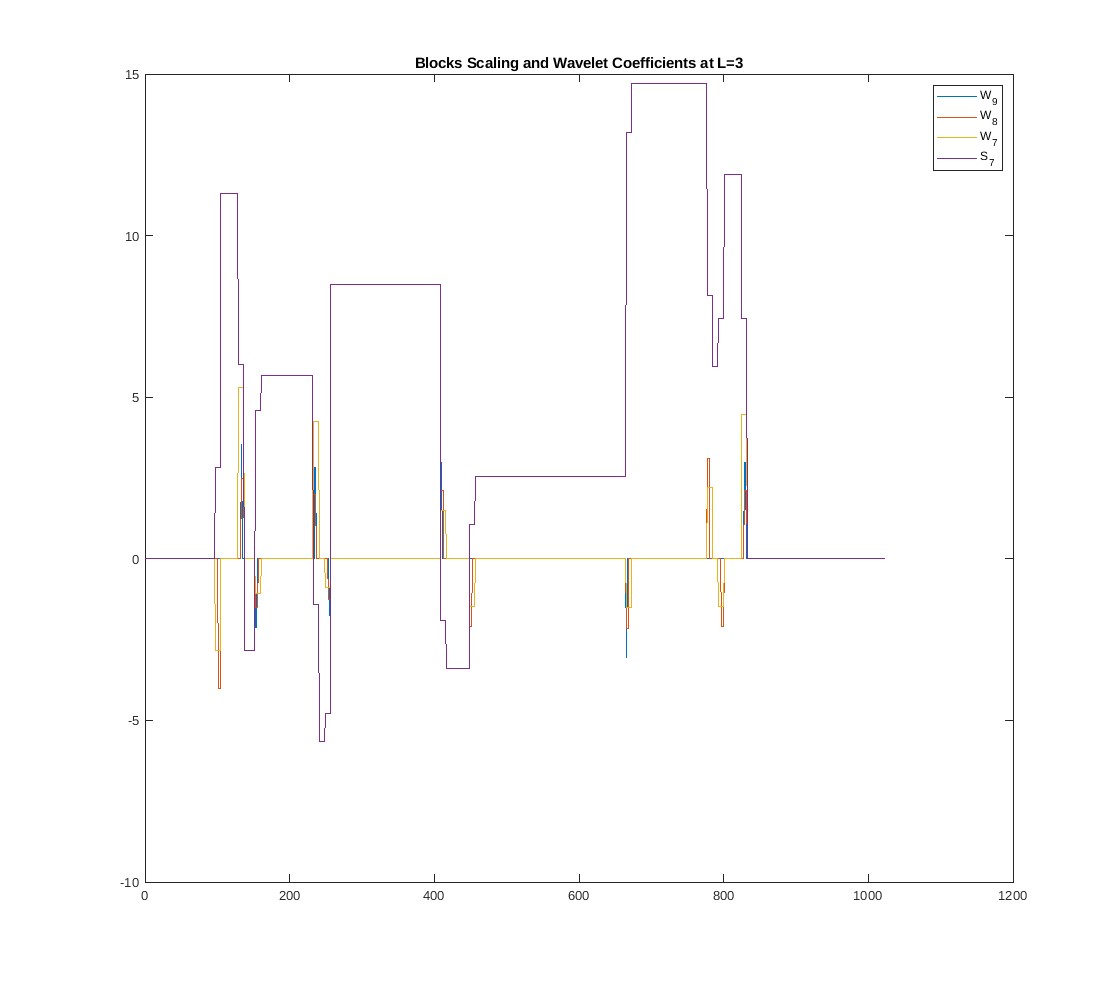
\includegraphics[scale=0.4]{6-2b.jpg}
\end{figure}



\newpage
\begin{tabbing}
    
\end{tabbing}
\newpage

\item[d.] Test with bumps.mat:
\begin{lstlisting}[language=matlab]
load("bumps.mat");
bumps = c;

w_bumps = haar(c, 3);
bumps_hat = ihaar(w_bumps, 3);

% Ensure Perfect Reconstruction
err = norm(bumps - bumps_hat)^2

% Ensure Energy is Conserved
signal_energy = norm(bumps)^2
transform_energy = norm(w_bumps)^2

h = ones(2,1);
w_9 = upsample(w_bumps(1:512), 2);
w_9 = conv(h.', w_9);

h = ones(4,1);
w_8 = upsample(w_bumps(513:768), 4);
w_8 = conv(h.', w_8);

h = ones(8,1);
w_7 = upsample(w_bumps(769:896), 8);
w_7 = conv(h.', w_7);
s_7 = upsample(w_bumps(897:end), 8);
s_7 = conv(h.', s_7);
plot(w_9(1:end-1)); hold on
plot(w_8(1:end-3));
plot(w_7(1:end-7));
plot(s_7(1:end-7)); 
legend({'W_9', 'W_8', 'W_7', 'S_7'}); 
title("Bumps Scaling and Wavelet Coefficients at L=3"); hold off
\end{lstlisting}

\begin{framed}
\[\|\text{bumps}-\hat{\text{bumps}}\|^2 = 0\]
\[\|\text{bumps}\|^2 = \|\text{Haar(bumps)}\|^2\]
\end{framed}

\begin{figure}[h]
    \caption{Bumps Wavelet Transform L=3}
    \centering
    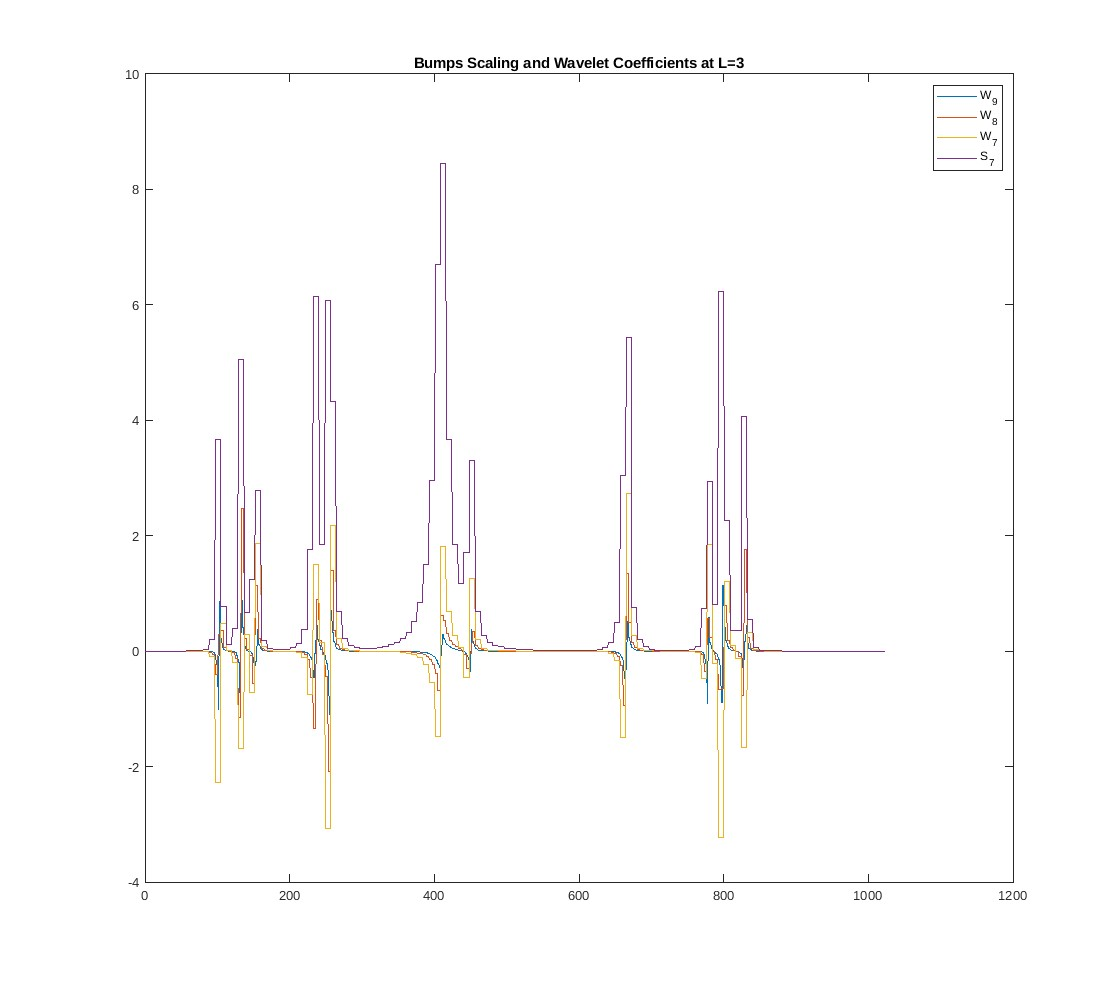
\includegraphics[scale=0.4]{6-2a.jpg}
\end{figure}

\end{enumerate}

\end{enumerate}


\end{document}
